\chapter{Specifikacija programske potpore}
		
	\section{Funkcionalni zahtjevi}
			
			\noindent \textbf{Dionici:}
			
			\begin{packed_enum}
				
				\item Donor
				\item Zavod
				\item Crveni Križ
				\item Administrator
				\item Razvojni tim ( Bruna Matić, Bruno Galić, Jana Matić, Jelena Lončar, Nikola Borzić, Nikola Marić, Zvonko Lelas )
				\item Asistent predmeta ( Mateja Golec )
				\item profesor predmeta ( Vlado Sruk )
				
			\end{packed_enum}
			
			\noindent \textbf{Aktori i njihovi funkcionalni zahtjevi:}
			
			
			\begin{packed_enum}
				\item  \underbar{Donor (sudionik) može:}
				
				\begin{packed_enum}
					
					\item pristupiti podacima
					\begin{packed_enum}
						
						\item pristup osobnim podacima (ime, prezime, krvna grupa)
						\item  pristupiti svojoj povijesti darivanja
						\item  pristupiti informacijama o akcijama
						\item pristupiti informacijama o količini krvi u pojedinim gradovima
						\item brisanje svog korisničkog računa
				
					\end{packed_enum}

					\item vidjeti koliki mu je period čekanja do sljedećeg darivanja
					\item prijava na akcije
					\item primanje obavijesti od zavoda u slučaju manjka krvi
					\item potvrđivanje pozivnica za darivanje
					\item pristup lokacijama na karti u kojima su organizirana doniranja krvi
					
				\end{packed_enum}
				\item  \underbar{Neregistrirani korisnik (sudionik) može:}
					\begin{packed_enum}
						
						\item vidjeti kartu lokacija za doniranje
						\item vidjeti akcije u kartici
						\item registrirati se
						\begin{packed_enum}
						
						\item kao donor
						\item  kao Crveni Križ
						\item  kao zavod
				
					\end{packed_enum}
				
					\end{packed_enum}
				\item  \underbar{Crveni Križ (inicijator) može:}
				
				\begin{packed_enum}
					
					\item izdavati akcije
					\item dodjeljivati priznanja (nagrade)
					\item evidencija darivatelja
					\item izdavanje potvrda
					\item davanje pozivnica
				\end{packed_enum}

				\item \underbar{Zavod (inicijator) može:}
				\begin{packed_enum}
					
					\item vidjeti popis donora
					\item brisati korisničke račune
					\item izdavati akcije
				\end{packed_enum}
			
				\item \underbar{Baza podataka (inicijator) može:}
				\begin{packed_enum}
					
					\item pohraniti sve podatke o donorima i njihovim ovlastima
					\item pohranjuje podatke o:
						\begin{packed_enum}
						
							\item lokacijama doniranja
							\item količinama krvi
							\item akcijama
							\item odzivima na akcije
						\end{packed_enum}
				\end{packed_enum}
			
			\end{packed_enum}
			
			\eject 
			
			
				
			\subsection{Obrasci uporabe}
				
				\subsubsection{Opis obrazaca uporabe}
				
					\noindent \underbar{\textbf{UC$<$1$>$ -$<$Registracija$>$}}
					\begin{packed_item}
	
						\item \textbf{Glavni sudionik: }$<$Neregistrirani korisnik$>$
						\item  \textbf{Cilj:} $<$Registracija$>$
						\item  \textbf{Sudionici:} $<$Baza podataka$>$
						\item  \textbf{Preduvjet:} $<$Korisnik nema registriran račun s mailom koji želi koristiti$>$
						\item  \textbf{Opis osnovnog tijeka:}
						
						\item[] \begin{packed_enum}
	
							\item $<$Upiši podatke(email, lozinka, godina rođenja, spol, težina, krvna grupa)$>$
							\item $<$Potvrdi podatke$>$
							\item $<$Podaci se provjeravaju u bazi podataka$>$
							\item $<$Podatci se spremaju u bazu podataka$>$
							\item $<$Korisnik je sada prijavljen na web stranici te ima mogućnosti kao i Donor$>$
						\end{packed_enum}
						
						\item  \textbf{Opis mogućih odstupanja:}
						
						\item[] \begin{packed_item}
	
							\item[3.a] $<$Email se već koristi$>$
							\item[3.b] $<$Osoba je premlada za darivanje krvi$>$
						\end{packed_item}
					\end{packed_item}
					
					% UC2 - Pregled mogućih nagrada za donore
					\noindent \underbar{\textbf{UC$<$2$>$ -$<$Pregled mogućih nagrada za donore$>$}}
					\begin{packed_item}
						
						\item \textbf{Glavni sudionik:} $<$Neregistrirani korisnik, Donor$>$
						\item \textbf{Cilj:} $<$Pregled nagrada koje možeš dobiti kao donor$>$
						\item \textbf{Sudionici:} $<$Baza podataka$>$
						\item \textbf{Opis osnovnog tijeka:}
						
						\begin{packed_enum}
							
							\item Korisnik odabire opciju za pregled mogućih nagrada
							\item Iz baze podataka povlače se ažurni podaci o nagradama koje donor može ostvariti
							\item Korisniku se prikazuju podaci
							
						\end{packed_enum}
						
					\end{packed_item}
					
					% UC3 - Pregled uvjeta za darivanje krvi
					\noindent \underbar{\textbf{UC$<$3$>$ -$<$Pregled uvjeta za darivanje krvi$>$}}
					\begin{packed_item}
						
						\item \textbf{Glavni sudionik:} $<$Neregistrirani korisnik, Donor$>$
						\item \textbf{Cilj:} $<$Pregled uvjeta koje moraš ispuniti da bi darivao krv$>$
						\item \textbf{Sudionici:} $<$Baza podataka$>$
						\item \textbf{Opis osnovnog tijeka:}
						
						\begin{packed_enum}
							
							\item Korisnik odabire opciju za pregled uvjeta
							\item Iz baze podataka povlače se ažurni podaci o uvjetima za darivanje krvi
							\item Korisniku se prikazuju podaci
							
						\end{packed_enum}
						
					\end{packed_item}
					
					% UC4 - Pregled statusa zaliha krvi
					\noindent \underbar{\textbf{UC$<$4$>$ -$<$Pregled statusa zaliha krvi$>$}}
					\begin{packed_item}
						
						\item \textbf{Glavni sudionik:} $<$Donor, Neregistrirani korisnik$>$
						\item \textbf{Cilj:} $<$Pregled količine krvi po krvnim grupama u zavodima$>$
						\item \textbf{Sudionici:} $<$Baza podataka$>$
						\item \textbf{Opis osnovnog tijeka:}
						
						\begin{packed_enum}
							
							\item Korisnik odabire zavod za koji želi vidjeti stanje
							\item Povlačimo aktualne podatke iz baze podataka
							\item Prikaz podataka
							
						\end{packed_enum}
						
					\end{packed_item}
					
					% UC5 - Pregled obavijesti o akcijama
					\noindent \underbar{\textbf{UC$<$5$>$ -$<$Pregled obavijesti o akcijama$>$}}
					\begin{packed_item}
						
						\item \textbf{Glavni sudionik:} $<$Donor, Neregistrirani korisnici$>$
						\item \textbf{Cilj:} $<$Pregled obavijesti$>$
						\item \textbf{Sudionici:} $<$Baza podataka$>$
						\item \textbf{Opis osnovnog tijeka:}
						
						\begin{packed_enum}
							
							\item Korisnik odabire stranicu za pregled obavijesti
							\item Povlačimo aktualne podatke iz baze podataka
							\item Korisnik može čitati podatke
							
						\end{packed_enum}
						
					\end{packed_item}
					
					% UC6 - Pregled karte RH s označenim lokacijama
					\noindent \underbar{\textbf{UC$<$6$>$ -$<$Pregled karte RH s označenim lokacijama$>$}}
					\begin{packed_item}
						
						\item \textbf{Glavni sudionik:} $<$Neregistrirani korisnik, Donor$>$
						\item \textbf{Cilj:} $<$Prikaz lokacija zavoda$>$
						\item \textbf{Sudionici:} $<$Baza podataka$>$
						\item \textbf{Opis osnovnog tijeka:}
						
						\begin{packed_enum}
							
							\item Korisnik odabire kartu
							\item Na karti Republike Hrvatske nalaze se lokacije gdje se može darivati krv
							\item Korisnik ima opciju odabrati pojedinu lokaciju te vidjeti stanje zavoda (UC$<$4$>$)
							
						\end{packed_enum}
						
					\end{packed_item}
					
					% UC7 - Prijava
					\noindent \underbar{\textbf{UC$<$7$>$ -$<$Prijava$>$}}
					\begin{packed_item}
						
						\item \textbf{Glavni sudionik:} $<$Donor$>$
						\item \textbf{Cilj:} $<$Prijava$>$
						\item \textbf{Sudionici:} $<$Baza podataka$>$
						\item \textbf{Preduvjet:} $<$Korisnik ima račun$>$
						\item \textbf{Opis osnovnog tijeka:}
						
						\begin{packed_enum}
							
							\item Unos emaila i lozinke
							\item Provjera u bazi podataka
							\item Korisnik je prebačen u način rada za Donora te je prijavljen
							
						\end{packed_enum}
						
						\item \textbf{Opis mogućih odstupanja:}
						
						\begin{packed_item}
							
							\item[3.a] Račun ne postoji
							\begin{enumerate}
								\item Prebacuje se na Registraciju
							\end{enumerate}
							\item[3.b] Kriva lozinka
							\begin{enumerate}
								\item Ponovi unos lozinke
							\end{enumerate}
							
						\end{packed_item}
						
					\end{packed_item}
					
					% UC8 - Odjava
					\noindent \underbar{\textbf{UC$<$8$>$ -$<$Odjava$>$}}
					\begin{packed_item}
						
						\item \textbf{Glavni sudionik:} $<$Donor$>$
						\item \textbf{Cilj:} $<$Odjava$>$
						\item \textbf{Preduvjet:} $<$Korisnik je prijavljen na web stranici$>$
						\item \textbf{Opis osnovnog tijeka:}
						
						\begin{packed_enum}
							
							\item Korisnik odabire opciju Odjavi se
							\item Korisnik biva odjavljen te ga se prebacuje u način rada za neregistriranog korisnika
							
						\end{packed_enum}
						
					\end{packed_item}
					
					% UC9 – Ažuriranje i pregled osobnih podataka
					\noindent \underbar{\textbf{UC$<$9$>$ -$<$Ažuriranje i pregled osobnih podataka$>$}}
					\begin{packed_item}
						
						\item \textbf{Glavni sudionik:} $<$Donor$>$
						\item \textbf{Cilj:} $<$Pregled i promjena osobnih podataka$>$
						\item \textbf{Sudionici:} $<$Baza podataka$>$
						\item \textbf{Preduvjet:} $<$Korisnik ima račun$>$
						\item \textbf{Opis osnovnog tijeka:}
						
						\begin{packed_enum}
							
							\item Korisnik odabire opciju Moj račun
							\item Iz baze podataka prikazujemo njegove podatke
							\item Korisnik može pregledavati svoje podatke
							\item Korisnik ima opciju uređivanja svojih podataka
							\item Nakon uređivanja potvrđuje promjene
							
						\end{packed_enum}
						
						\item \textbf{Opis mogućih odstupanja:}
						
						\begin{packed_item}
							
							\item[5.a] Nedozvoljene promjene (korisnik nije punoljetan)
							\begin{enumerate}
								\item Javlja se greška te se pita korisnika je li to njegov stvarni datum rođenja
								\item Ako nije, odbacuju se promjene
								\item Ako je, račun se briše te se obavještava korisnika
								
							\end{enumerate}
							
						\end{packed_item}
						
					\end{packed_item}
					
					% UC10 – Pregled povijesti darivanja
					\noindent \underbar{\textbf{UC$<$10$>$ -$<$Pregled povijesti darivanja$>$}}
					\begin{packed_item}
						
						\item \textbf{Glavni sudionik:} $<$Donor$>$
						\item \textbf{Cilj:} $<$Pregled povijesti darivanja$>$
						\item \textbf{Sudionici:} $<$Baza podataka$>$
						\item \textbf{Opis osnovnog tijeka:}
						
						\begin{packed_enum}
							
							\item Korisnik odabire opciju Povijest darivanja
							\item Prikazuju se ažurni podaci iz baze podataka o svim darivanjima krvi
							\item Korisnik ima opciju izdavanja potvrde za pojedinu donaciju (UC$<$12$>$)
							
						\end{packed_enum}
						
					\end{packed_item}
					
					% UC11 – Prijavljivanje za darivanje krvi
					\noindent \underbar{\textbf{UC$<$11$>$ -$<$Prijavljivanje za darivanje krvi$>$}}
					\begin{packed_item}
						
						\item \textbf{Glavni sudionik:} $<$Donor$>$
						\item \textbf{Cilj:} $<$Rezervacija termina za doniranje krvi$>$
						\item \textbf{Sudionici:} $<$Baza podataka, Zavod$>$
						\item \textbf{Preduvjet:} $<$Prošlo je dovoljno vremena od zadnje donacije, korisnik nije prijavio ništa izvanredno (bolest, tetovaže…)$>$
						\item \textbf{Opis osnovnog tijeka:}
						
						\begin{packed_enum}
							
							\item Korisnik odabire opciju Rezervacija (za određeni zavod)
							\item Iz baze podataka prikazujemo podatke (slobodni termini)
							\item Korisnik odabire slobodni termin
							\item Korisnik potvrđuje dolazak na odabrani termin
							\item Termin se sprema u bazu podataka te se obavještava zavod
							
						\end{packed_enum}
						
						\item \textbf{Opis mogućih odstupanja:}
						
						\begin{packed_item}
							
							\item[4.a] U međuvremenu, za vrijeme rezerviranja, termin je popunjen
							\begin{enumerate}
								\item Obavještava se korisnika o neuspjehu rezervacije te se ponovno nudi mogućnost rezervacije
							\end{enumerate}
							
						\end{packed_item}
						
					\end{packed_item}
					
					% UC12 – Ispis potvrda i zahtjev za nagradama
					\noindent \underbar{\textbf{UC$<$12$>$ -$<$Ispis potvrda i zahtjev za nagradama$>$}}
					\begin{packed_item}
						
						\item \textbf{Glavni sudionik:} $<$Donor$>$
						\item \textbf{Cilj:} $<$Izdavanje potvrda o darivanju, bonusa i ispričnica$>$
						\item \textbf{Sudionici:} $<$Baza podataka$>$
						\item \textbf{Opis osnovnog tijeka:}
						
						\begin{packed_enum}
							
							\item Korisnik odabire opciju Dokumenti
							\item Prikazuju se termini na kojima je potvrđen dolazak Donora
							\item Korisnik odabire termin te ima opciju preuzimanja Potvrde o darivanju ili Ispričnice
							\item Ako je korisnik ostvario bonuse, također ima opciju preuzeti iste
							
						\end{packed_enum}
						
					\end{packed_item}
					
					% UC13 – Brisanje korisničkog računa
					\noindent \underbar{\textbf{UC$<$13$>$ -$<$Brisanje korisničkog računa$>$}}
					\begin{packed_item}
						
						\item \textbf{Glavni sudionik:} $<$Donor$>$
						\item \textbf{Cilj:} $<$Brisanje korisničkog računa$>$
						\item \textbf{Sudionici:} $<$Baza podataka$>$
						\item \textbf{Opis osnovnog tijeka:}
						
						\begin{packed_enum}
							
							\item Korisnik odabire opciju Obriši račun
							\item Korisnika se pita je li siguran da želi obrisati račun
							\item Korisnik potvrđuje te račun biva obrisan iz baze podataka zajedno sa svim podacima o računu
							\item Korisnik biva prebačen u način rada za Neregistriranog korisnika
							
						\end{packed_enum}
						
					\end{packed_item}
					
					% UC14 – Prijavljivanje za obavještavanje
					\noindent \underbar{\textbf{UC$<$14$>$ -$<$Prijavljivanje za obavještavanje$>$}}
					\begin{packed_item}
						
						\item \textbf{Glavni sudionik:} $<$Donor$>$
						\item \textbf{Cilj:} $<$Subscription na email listu$>$
						\item \textbf{Sudionici:} $<$Baza podataka$>$
						\item \textbf{Opis osnovnog tijeka:}
						
						\begin{packed_enum}
							
							\item Korisnik odabire da želi primati obavijesti
							\item Korisnik se stavlja na email listu
							\item Svaka obavijest koja dolazi na web stranicu također se šalje svima sa email liste
							\item Korisnik također ima opciju odjave s email liste
							
						\end{packed_enum}
						
					\end{packed_item}
					
					% UC15 – Registracija kao CK/Zavod
					\noindent \underbar{\textbf{UC$<$15$>$ -$<$Registracija kao CK/Zavod$>$}}
					\begin{packed_item}
						
						\item \textbf{Glavni sudionik:} $<$Zavod, Crveni Križ$>$
						\item \textbf{Cilj:} $<$Registracija$>$
						\item \textbf{Sudionici:} $<$Baza podataka, Zavod, Crveni Križ$>$
						\item \textbf{Opis osnovnog tijeka:}
						
						\begin{packed_enum}
							
							\item Korisnik odabire opciju registracije kao Zavod/CK
							\item Korisnik unosi podatke te čeka potvrdu
							\item U slučaju da se registrira kao Zavod, može ga potvrditi samo taj Zavod za koji se registrira ili Crveni Križ
							\item U slučaju da se registrira kao Crveni Križ, može ga potvrditi samo Crveni Križ
							\item Kada biva potvrđen, dobiva obavijest na email
							
						\end{packed_enum}
						
					\end{packed_item}
					
					% UC16 – Uvid u popis donora
					\noindent \underbar{\textbf{UC$<$16$>$ -$<$Uvid u popis donora$>$}}
					\begin{packed_item}
						
						\item \textbf{Glavni sudionik:} $<$Zavod, Crveni Križ$>$
						\item \textbf{Cilj:} $<$Pregled donora$>$
						\item \textbf{Sudionici:} $<$Baza podataka$>$
						\item \textbf{Opis osnovnog tijeka:}
						
						\begin{packed_enum}
							
							\item Korisnik odabire opciju Pregled donora
							\item Korisnik dobiva popis svih donora te pregled njihovih podataka (ne baš svih)
							
						\end{packed_enum}
						
					\end{packed_item}
					
					% UC17 – Objava akcija darivanja krvi
					\noindent \underbar{\textbf{UC$<$17$>$ -$<$Objava akcija darivanja krvi$>$}}
					\begin{packed_item}
						
						\item \textbf{Glavni sudionik:} $<$Zavod, Crveni Križ$>$
						\item \textbf{Cilj:} $<$Objava akcija$>$
						\item \textbf{Sudionici:} $<$Donor, Neregistrirani korisnik$>$
						\item \textbf{Opis osnovnog tijeka:}
						
						\begin{packed_enum}
							
							\item Korisnik ima opciju objaviti akciju (postaviti objavu) koju će vidjeti svi Korisnici (Donori i Neregistrirani korisnici)
							\item Objava se također šalje svima prijavljenima na email listu
							
						\end{packed_enum}
						
					\end{packed_item}
					
					% UC18 – Komunikacija s Donorima
					\noindent \underbar{\textbf{UC$<$18$>$ -$<$Komunikacija s Donorima$>$}}
					\begin{packed_item}
						
						\item \textbf{Glavni sudionik:} $<$Crveni Križ, Zavod$>$
						\item \textbf{Cilj:} $<$Komunikacija s Donorima$>$
						\item \textbf{Sudionici:} $<$Donor$>$
						\item \textbf{Opis osnovnog tijeka:}
						
						\begin{packed_enum}
							
							\item Korisnik šalje hitnu obavijest svima ili određenim krvnim grupama zbog nestašice krvi
							
						\end{packed_enum}
						
					\end{packed_item}
					
					% UC19 – Pregled statistike o donacijama
					\noindent \underbar{\textbf{UC$<$19$>$ -$<$Pregled statistike o donacijama$>$}}
					\begin{packed_item}
						
						\item \textbf{Glavni sudionik:} $<$Zavod, Crveni Križ$>$
						\item \textbf{Cilj:} $<$Pregled statistike$>$
						\item \textbf{Sudionici:} $<$Baza podataka$>$
						\item \textbf{Opis osnovnog tijeka:}
						
						\begin{packed_enum}
							
							\item Korisnik odabire opciju Statistika
							\item Računa se ažurna statistika iz baze podataka
							\item Zavodima se prikazuje statistika samo za njihov zavod
							\item Crveni Križ vidi statistiku svih zavoda
							
						\end{packed_enum}
						
					\end{packed_item}
					
					% UC20 – Izdavanje potvrda
					\noindent \underbar{\textbf{UC$<$20$>$ -$<$Izdavanje potvrda$>$}}
					\begin{packed_item}
						
						\item \textbf{Glavni sudionik:} $<$Crveni Križ$>$
						\item \textbf{Cilj:} $<$Izdavanje potvrda o darivanju, bonusa i ispričnica$>$
						\item \textbf{Sudionici:} $<$Baza podataka$>$
						\item \textbf{Opis osnovnog tijeka:}
						
						\begin{packed_enum}
							
							\item Korisnik može potvrditi zahtjev za potvrdu
							
						\end{packed_enum}
						
					\end{packed_item}
					
					% UC21 – Verifikacija podataka
					\noindent \underbar{\textbf{UC$<$21$>$ -$<$Verifikacija podataka$>$}}
					\begin{packed_item}
						
						\item \textbf{Glavni sudionik:} $<$Crveni Križ$>$
						\item \textbf{Cilj:} $<$Verifikacija podataka$>$
						\item \textbf{Sudionici:} $<$Baza podataka$>$
						\item \textbf{Opis osnovnog tijeka:}
						
						\begin{packed_enum}
							
							\item Korisnik može verificirati podatke Donora
							\item Korisnik može potvrditi i odbiti registraciju za Zavod/Crveni Križ
							
						\end{packed_enum}
						
					\end{packed_item}
					
					% UC22 – Brisanje donorskih korisničkih računa
					\noindent \underbar{\textbf{UC$<$22$>$ -$<$Brisanje donorskih korisničkih računa$>$}}
					\begin{packed_item}
						
						\item \textbf{Glavni sudionik:} $<$Crveni Križ$>$
						\item \textbf{Cilj:} $<$Brisanje računa$>$
						\item \textbf{Sudionici:} $<$Baza podataka, Donor$>$
						\item \textbf{Opis osnovnog tijeka:}
						
						\begin{packed_enum}
							
							\item Korisnik odabire opciju Brisanja korisničkog računa
							\item Korisnik mora napisati razlog brisanja korisničkog računa
							\item Korisnički račun se briše iz baze podataka, te se pohranjuje da je račun obrisan i razlog brisanja
							
						\end{packed_enum}
						
					\end{packed_item}
					
					% UC23 – Dodjela priznanja
					\noindent \underbar{\textbf{UC$<$23$>$ -$<$Dodjela priznanja$>$}}
					\begin{packed_item}
						
						\item \textbf{Glavni sudionik:} $<$Crveni Križ$>$
						\item \textbf{Cilj:} $<$Dodjela priznanja$>$
						\item \textbf{Sudionici:} $<$Donor$>$
						\item \textbf{Opis osnovnog tijeka:}
						
						\begin{packed_enum}
							
							\item Korisnik odabire Donora
							\item Korisnik ima mogućnost dodijeliti Donoru posebno priznanje zbog njegovog doprinosa
							\item Korisnik upisuje priznanje koje će Donor dobiti
							\item Donor biva obavješten o priznanju koje je dobio
							
						\end{packed_enum}
						
					\end{packed_item}
					
					% UC24 – Upravljanje aplikacijom
					\noindent \underbar{\textbf{UC$<$24$>$ -$<$Upravljanje aplikacijom$>$}}
					\begin{packed_item}
						
						\item \textbf{Glavni sudionik:} $<$Admin$>$
						\item \textbf{Cilj:} $<$Upravljanje aplikacijom$>$
						\item \textbf{Opis osnovnog tijeka:}
						
						\begin{packed_enum}
							
							\item Admin ima pristup serveru te može mijenjati datoteke u serveru
							
						\end{packed_enum}
						
					\end{packed_item}
					
					% UC25 – Upravljanje korisničkim računima
					\noindent \underbar{\textbf{UC$<$25$>$ -$<$Upravljanje korisničkim računima$>$}}
					\begin{packed_item}
						
						\item \textbf{Glavni sudionik:} $<$Admin$>$
						\item \textbf{Cilj:} $<$Pregled, brisanje, ažuriranje korisničkih računa$>$
						\item \textbf{Sudionici:} $<$Baza podataka$>$
						\item \textbf{Opis osnovnog tijeka:}
						
						\begin{packed_enum}
							
							\item Admin može upravljati korisničkim računima
							
						\end{packed_enum}
						
					\end{packed_item}
					
					% UC26 – Upravljanje pravima pristupa
					\noindent \underbar{\textbf{UC$<$26$>$ -$<$Upravljanje pravima pristupa$>$}}
					\begin{packed_item}
						
						\item \textbf{Glavni sudionik:} $<$Admin$>$
						\item \textbf{Cilj:} $<$Promjena prava pristupa$>$
						\item \textbf{Opis osnovnog tijeka:}
						
						\begin{packed_enum}
							
							\item Admin može bilo kome oduzeti odnosno dodijeliti pravo pristupa nekim podacima
							
						\end{packed_enum}
						
					\end{packed_item}
					
					% UC27 – Praćenje performansi
					\noindent \underbar{\textbf{UC$<$27$>$ -$<$Praćenje performansi$>$}}
					\begin{packed_item}
						
						\item \textbf{Glavni sudionik:} $<$Admin$>$
						\item \textbf{Cilj:} $<$Praćenje performansi$>$
						\item \textbf{Opis osnovnog tijeka:}
						
						\begin{packed_enum}
							
							\item Admin može pratiti performanse sustava (broj pristupa stranici, vrijeme odziva servera…)
							
						\end{packed_enum}
						
					\end{packed_item}
					
					% UC28 – Postavljanje i održavanje sigurnosti
					\noindent \underbar{\textbf{UC$<$28$>$ -$<$Postavljanje i održavanje sigurnosti$>$}}
					\begin{packed_item}
						
						\item \textbf{Glavni sudionik:} $<$Admin$>$
						\item \textbf{Cilj:} $<$Sigurnost$>$
						\item \textbf{Opis osnovnog tijeka:}
						
						\begin{packed_enum}
							
							\item Admin može vidjeti postoje li napadi na web stranicu te reagirati sukladno prijetnji
							
						\end{packed_enum}
						
					\end{packed_item}
					
					% UC29 – Kreiranje i uređivanje sadržaja na web stranici
					\noindent \underbar{\textbf{UC$<$29$>$ -$<$Kreiranje i uređivanje sadržaja na web stranici$>$}}
					\begin{packed_item}
						
						\item \textbf{Glavni sudionik:} $<$Admin$>$
						\item \textbf{Cilj:} $<$Uređivanje web stranice$>$
						\item \textbf{Opis osnovnog tijeka:}
						
						\begin{packed_enum}
							
							\item Admin može mijenjati izgled web stranice
							
						\end{packed_enum}
						
					\end{packed_item}
					
				\subsubsection{Dijagrami obrazaca uporabe}
					
					\begin{figure}[H]
						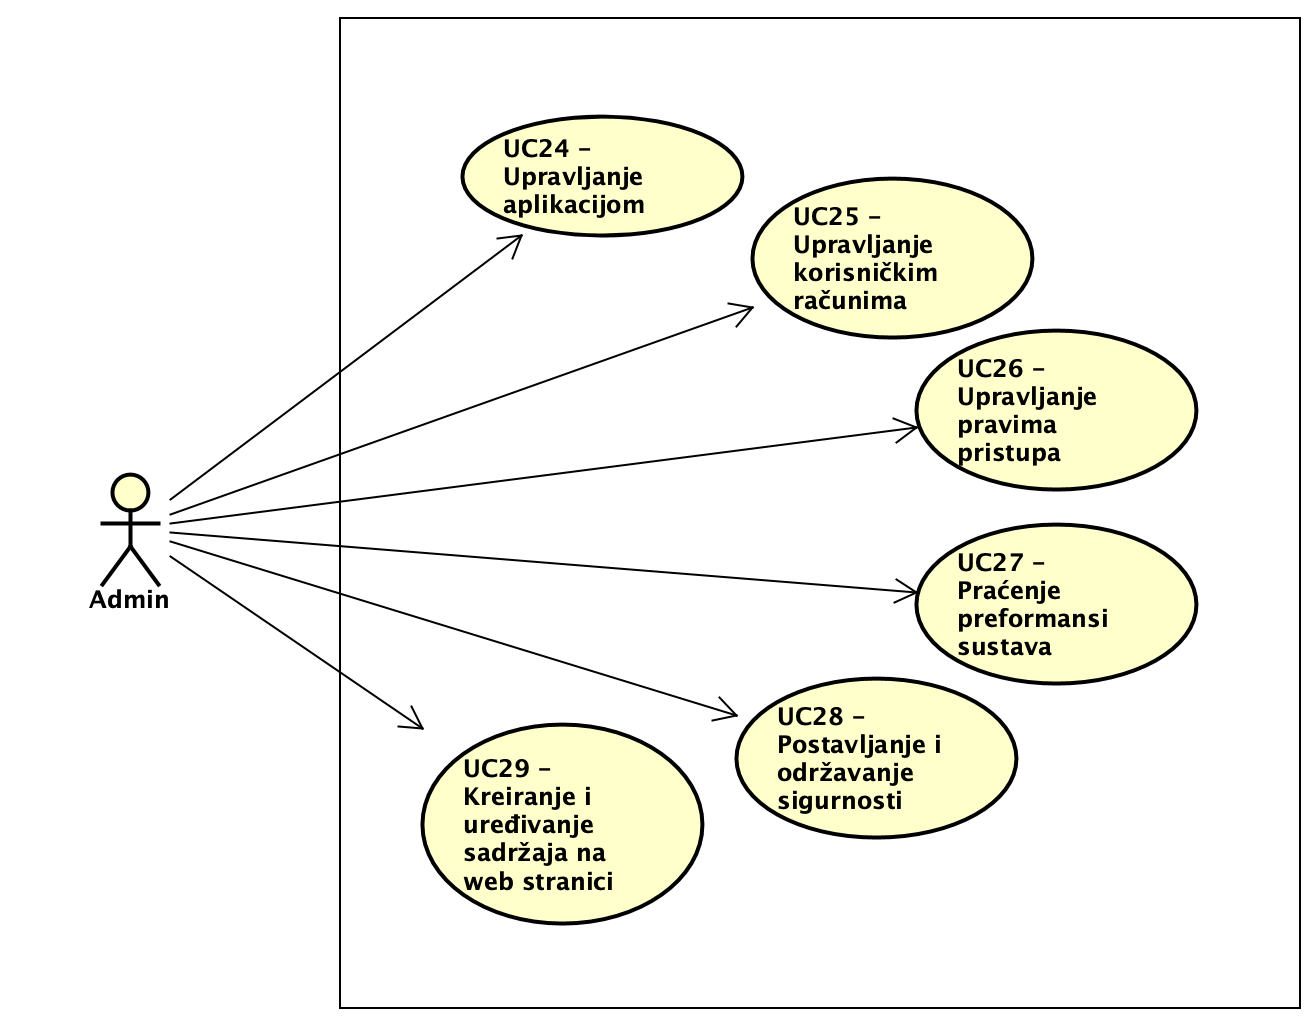
\includegraphics[scale=0.4]{slike/Dijagrami/DOU_admin.PNG} %veličina slike u odnosu na originalnu datoteku i pozicija slike
						\centering
						\caption{Dijagram uporabe obrazaca za admina}
						\label{fig:promjene}
					\end{figure}
					\begin{figure}[H]
						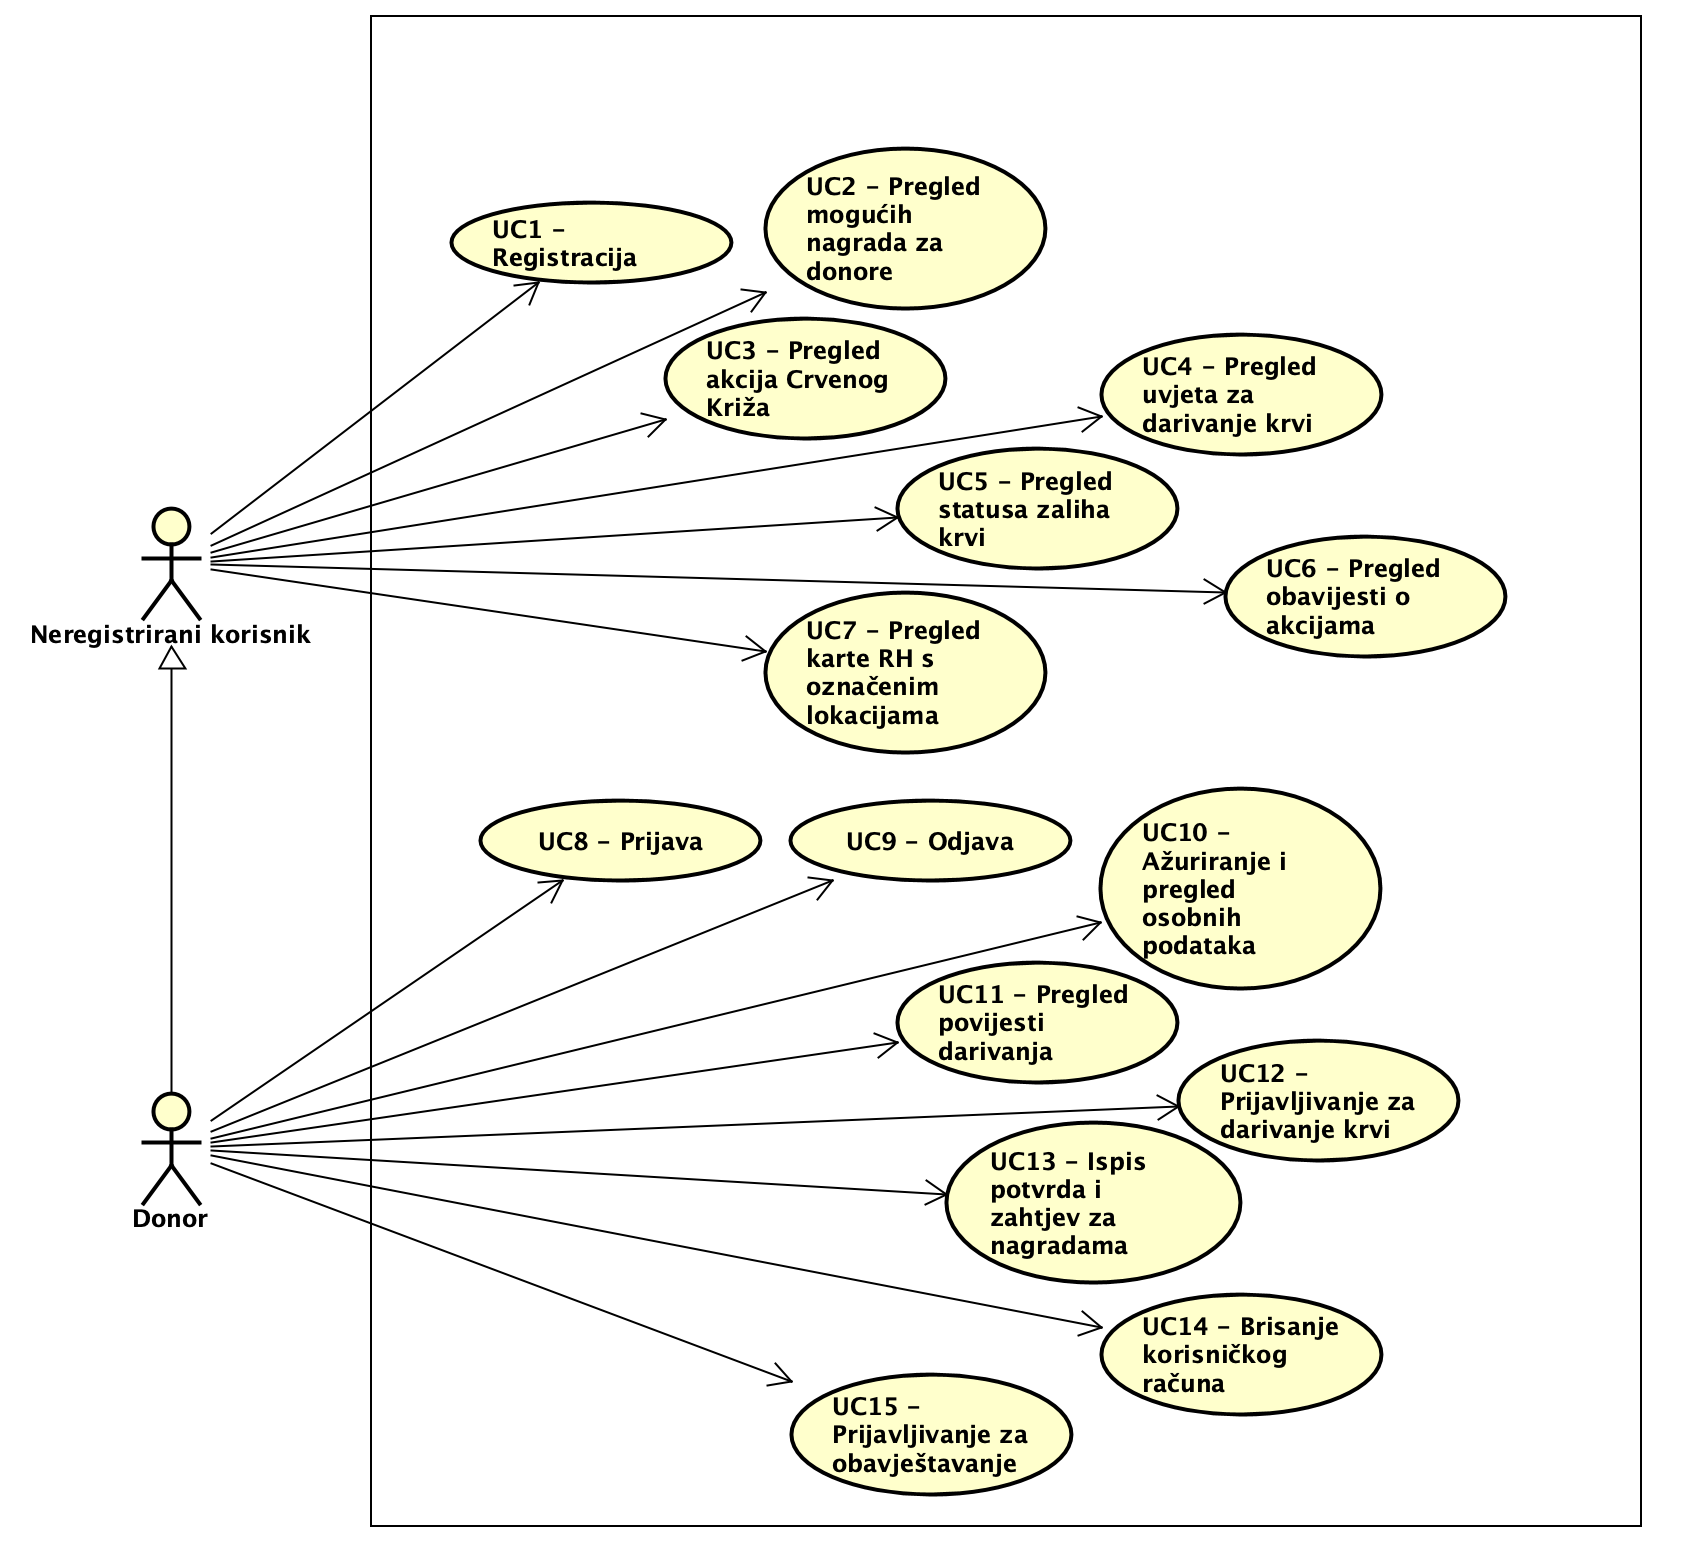
\includegraphics[scale=0.4]{slike/Dijagrami/DOU_donor.PNG} %veličina slike u odnosu na originalnu datoteku i pozicija slike
						\centering
						\caption{Dijagram uporabe obrazaca za donora}
						\label{fig:promjene}
					\end{figure}
					\begin{figure}[H]
						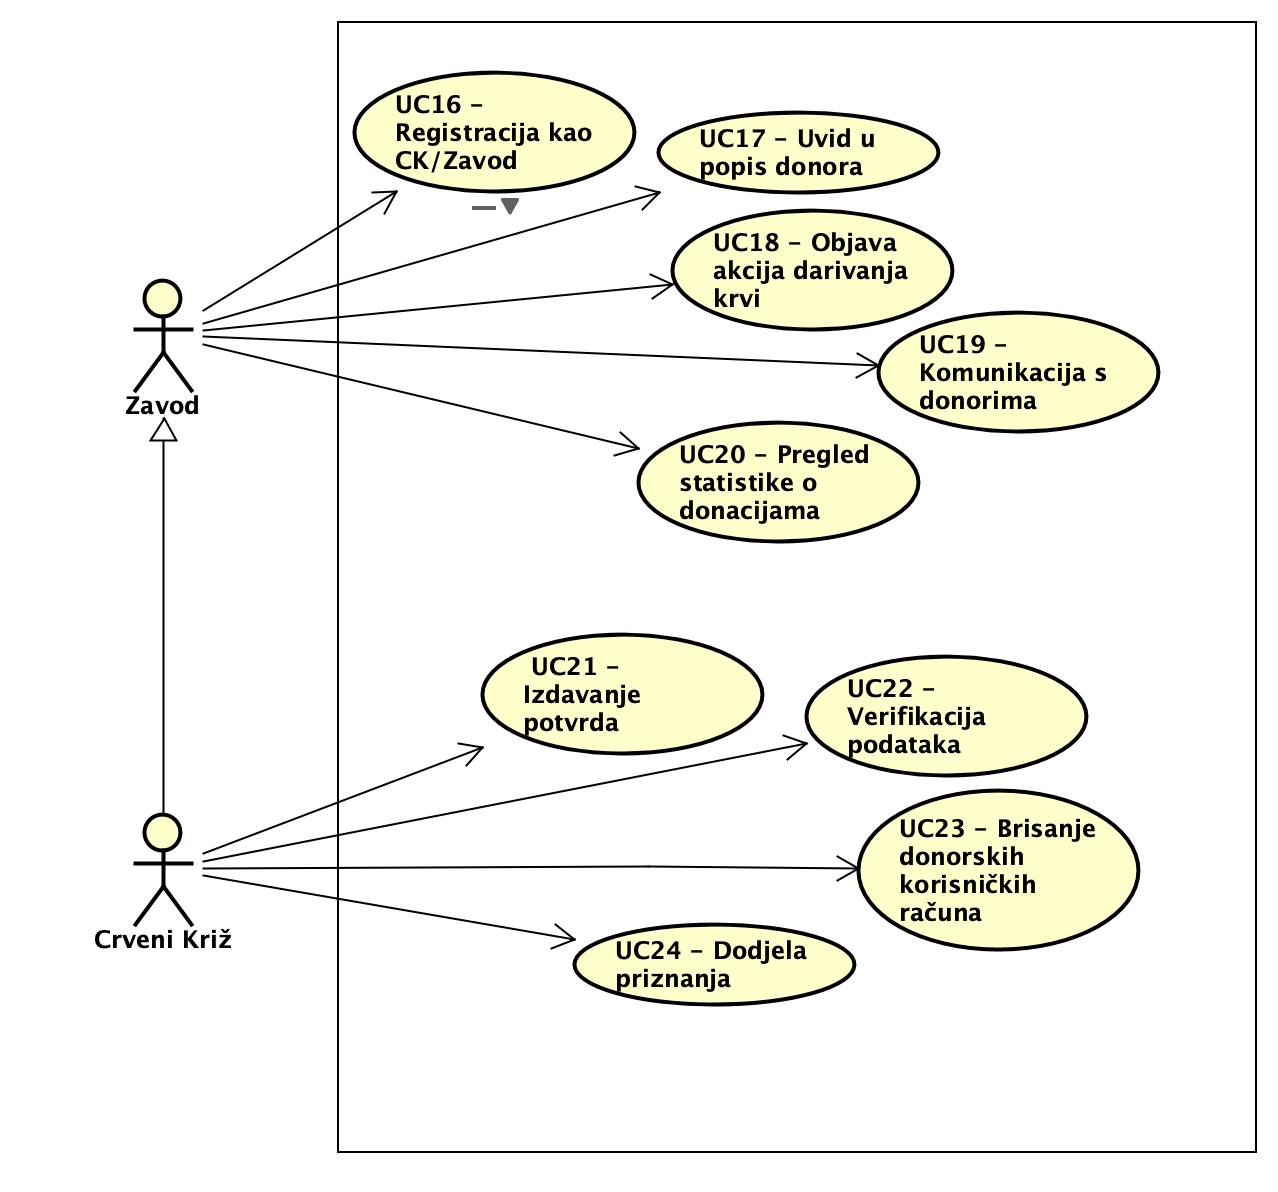
\includegraphics[scale=0.4]{slike/Dijagrami/DOU_zavod.PNG} %veličina slike u odnosu na originalnu datoteku i pozicija slike
						\centering
						\caption{Dijagram uporabe obrazaca za zavod}
						\label{fig:promjene}
					\end{figure}
				\eject		
				
			\subsection{Sekvencijski dijagrami}
				
				\textit{Nacrtati sekvencijske dijagrame koji modeliraju najvažnije dijelove sustava (max. 4 dijagrama). Ukoliko postoji nedoumica oko odabira, razjasniti s asistentom. Uz svaki dijagram napisati detaljni opis dijagrama.}
				\begin{figure}[H]
					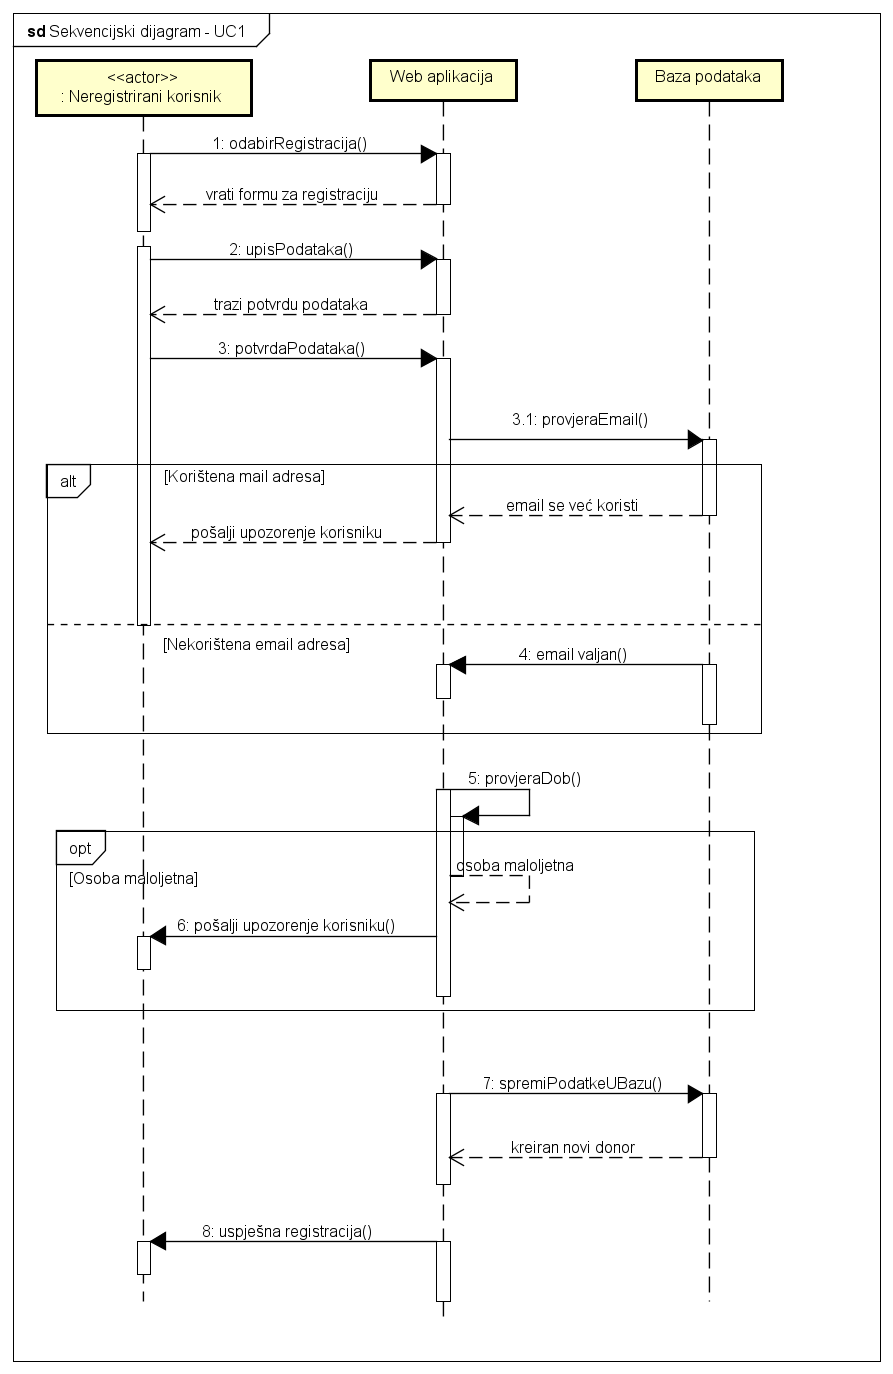
\includegraphics[scale=0.4]{slike/Dijagrami/Sekvencijski dijagram - UC1} %veličina slike u odnosu na originalnu datoteku i pozicija slike
					\centering
					\caption{Sekvencijski dijagram UC1}
					\label{fig:promjene}
				\end{figure}
				\begin{figure}[H]
					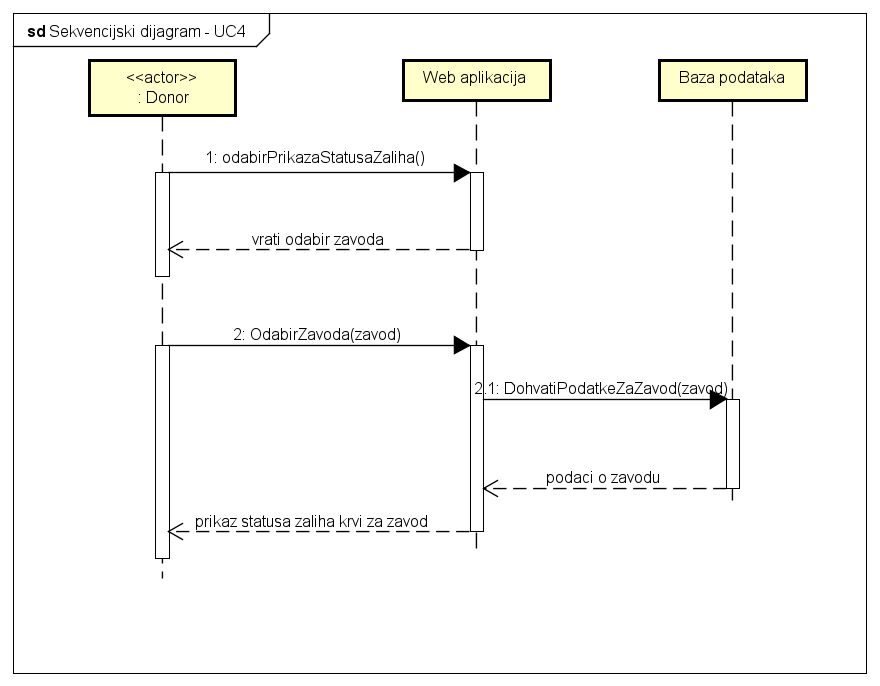
\includegraphics[scale=0.4]{slike/Dijagrami/Sekvencijski dijagram - UC4} %veličina slike u odnosu na originalnu datoteku i pozicija slike
					\centering
					\caption{Sekvencijski dijagram UC4}
					\label{fig:promjene}
				\end{figure}
				\begin{figure}[H]
					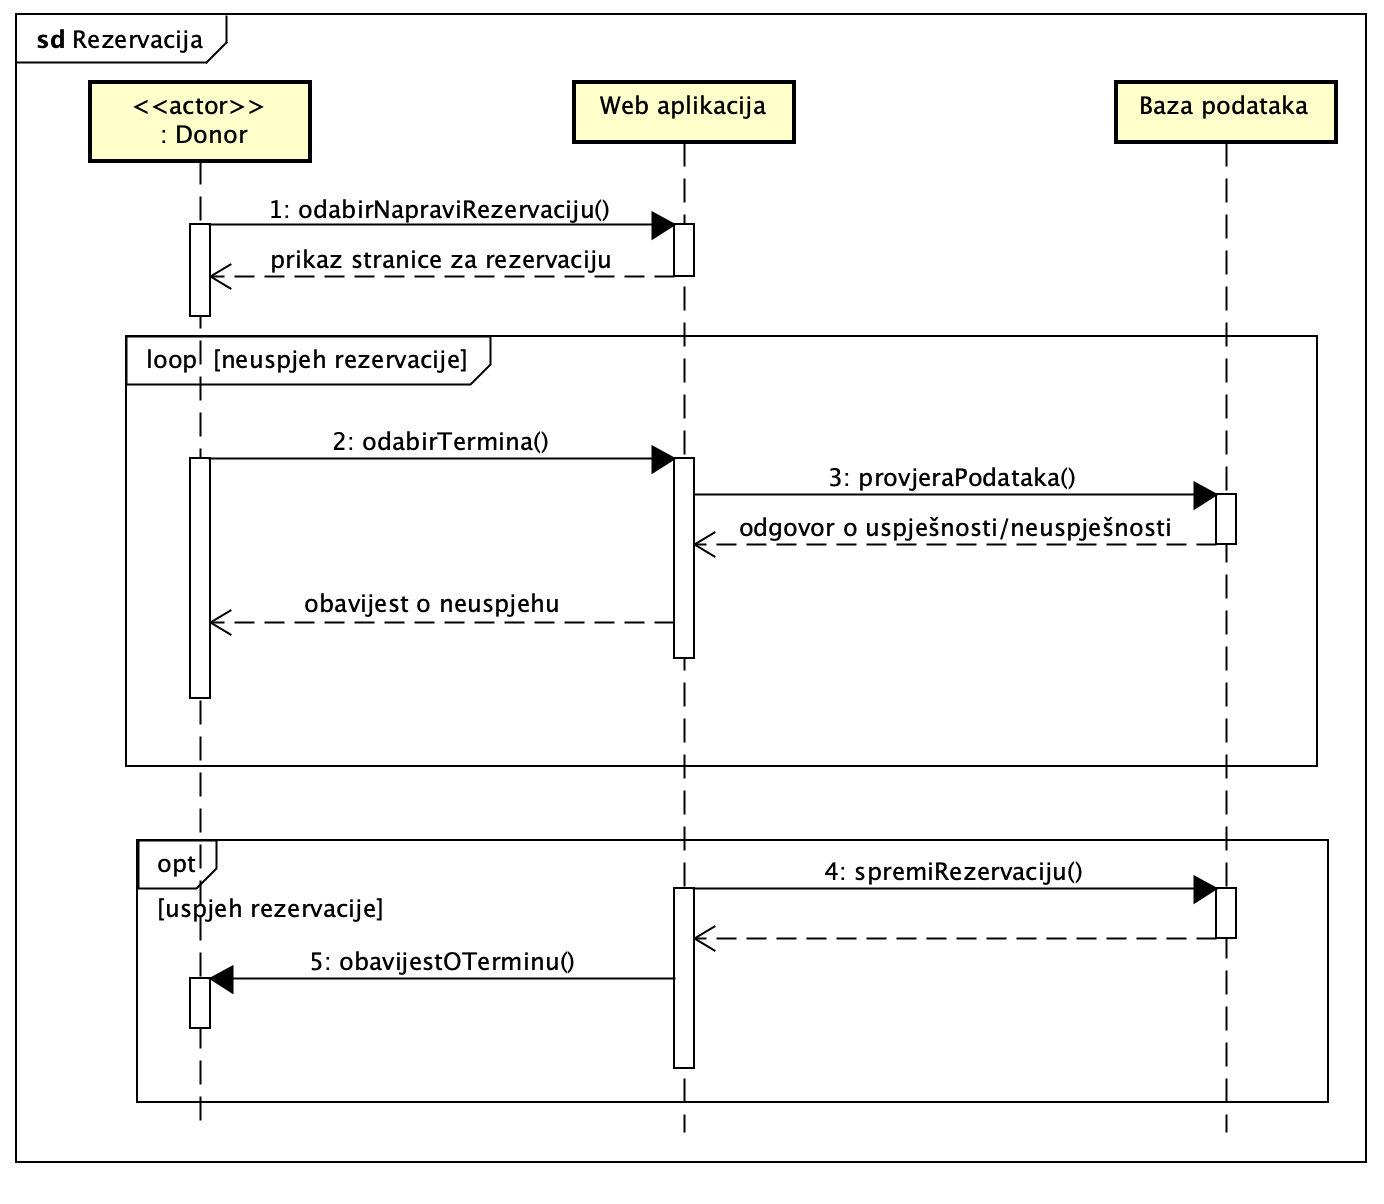
\includegraphics[scale=0.4]{slike/Dijagrami/Sekvencijski dijagram - UC11} %veličina slike u odnosu na originalnu datoteku i pozicija slike
					\centering
					\caption{Sekvencijski dijagram UC11}
					\label{fig:promjene}
				\end{figure}
				\begin{figure}[H]
					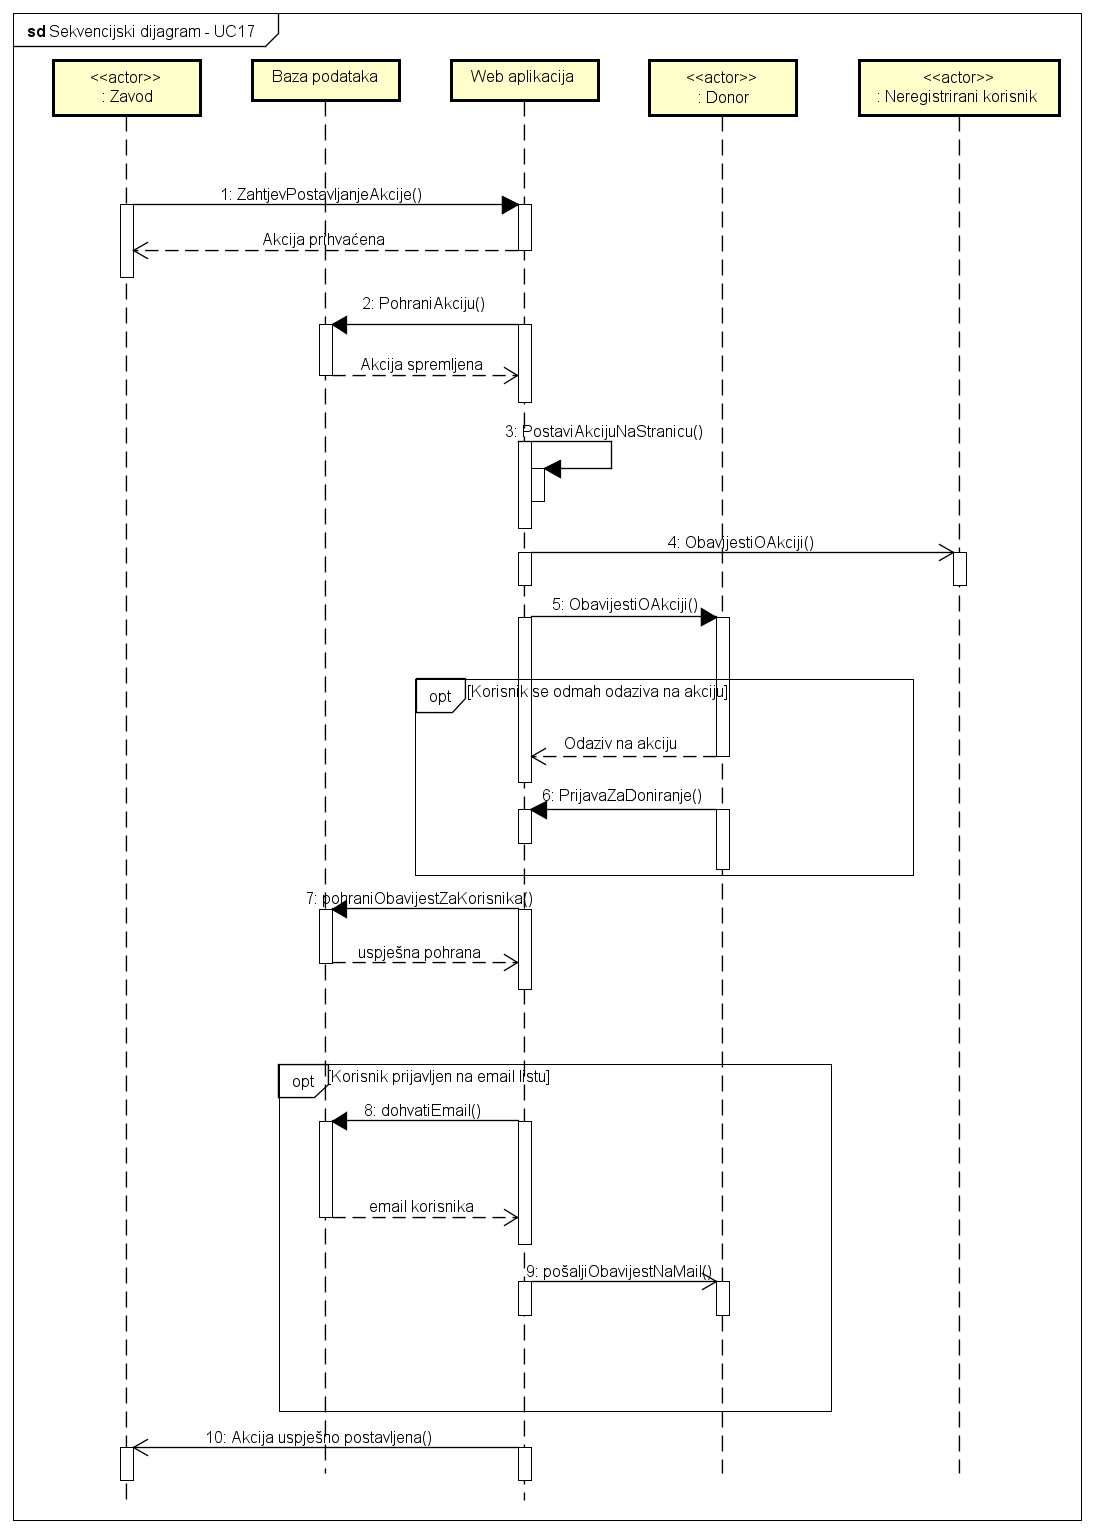
\includegraphics[scale=0.4]{slike/Dijagrami/Sekvencijski dijagram - UC17} %veličina slike u odnosu na originalnu datoteku i pozicija slike
					\centering
					\caption{Sekvencijski dijagram UC71}
					\label{fig:promjene}
				\end{figure}
				\eject
	
		\section{Ostali zahtjevi}
		
			\begin{packed_item}

				\item Sustav treba podržavati rad više korisnika u stvarnom vremenu
				\item Sustav treba biti izveden kao web aplikacija ispravno funkcionalna u svim web preglednicima
				\item	 Sustavu pristupaju registrirani korisnici pomoću korisničkog imena i pouzdane lozinke
				\item Sustav treba koristiti srednjoeuropsko strandardno vrijeme, GTM+1
				\item Sustav treba biti jednostavan i razumljiv svim korisnicima bez detaljnih uputa
				\item Sustav treba podržavati hrvatsku abecedu, uključujući dijakritičke znakove
				\item Na klijentskoj strani potrebno je implementirati korisničko sučelje koristeći React
				\item Na poslužiteljskoj strani je potrebno koristiti radni okvir Sequlize
				\item Podatke treba spremati u bazu podataka koristeći SQL?
				\item Sustav treba koristiti srednjoeuropsko strandardno vrijeme, GTM+1
				\item Sustav treba biti jednostavan i razumljiv svim korisnicima bez detaljnih uputa
				\item Sustav treba podržavati hrvatsku abecedu, uključujući dijakritičke znakove
			\end{packed_item}

			 
			 
	